\section{Architecture de l'application}
Comme susmentionné, l'architecture utilisée dans notre projet est l'architecture client-serveur.
Cette architecture nous permet de faire le lien entre le serveur de notre plateforme, et  l’éditeur de modèle de données d’une part, et la partie client et le serveur d’une autre part à l'aide de REST API.\\
Ci-dessous, le diagramme exposant l'architecture adoptée:
\begin{figure}[h!]  
 \centering
    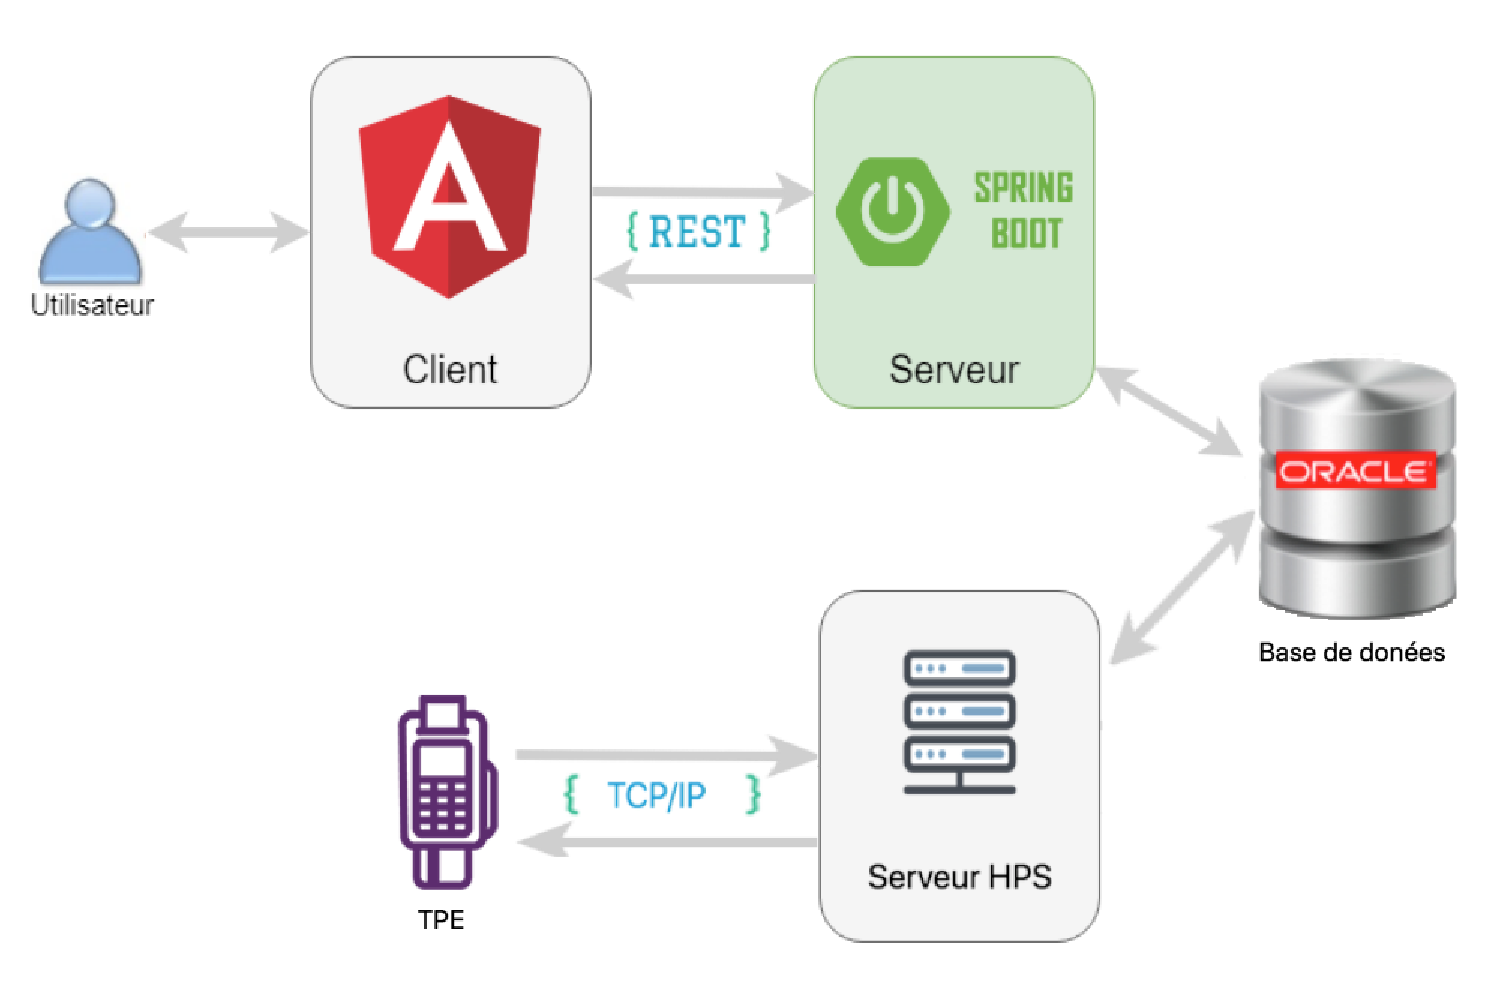
\includegraphics[width=0.8\textwidth]{chapitre3/Figures/archGenral.png}
  \caption{L'architecture technique de l'application}
\end{figure}
\subsection{Architecture Client}
Front-end qui est souvent appelé un client est un code qui s'exécute dans un navigateur. Il est responsable de la partie présentation (interface utilisateur). Dans Angular, nous utilisons HTML, CSS et Typescript pour créer une interface de notre application.
Le Front-end est responsable de l'affichage des données et de la logique de présentation.\\
La figure ci-dessous représente la description de l'architecture client :
\begin{figure}[h!]  
 \centering
    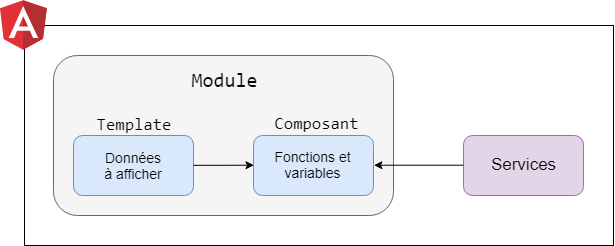
\includegraphics[width=0.8\textwidth]{chapitre3/Figures/angular.png}
  \caption{L'architecture client}
\end{figure}
\\
L'application est organisée en modules, un module est un bloc de code qui est conçu pour effectuer une seule tâche groupant des composants ainsi que des services, de manière à pouvoir les combiner avec d'autres modules pour créer une application.\\
Un composant est une classe qui gère la vue de l'application et contient la logique de base de la page. Chaque composant fait appel à un service qui est une fonction ou un objet qui peut être utilisé pour partager les données et le comportement à travers l'application en faisant appel au serveur.\\
Un template contient le code HTML du composant qui sera présenté à l’utilisateur.


\subsection{Architecture Serveur}
La partie serveur, aussi connu sous le nom Back-end, gère la réception des requêtes provenant du client, lance le module de gestion de données, gère les flux des requêtes et renvoie les résultats des requêtes au client.\\
La figure ci-dessous représente la description de l'architecture serveur :
\begin{figure}[h!]  
 \centering
    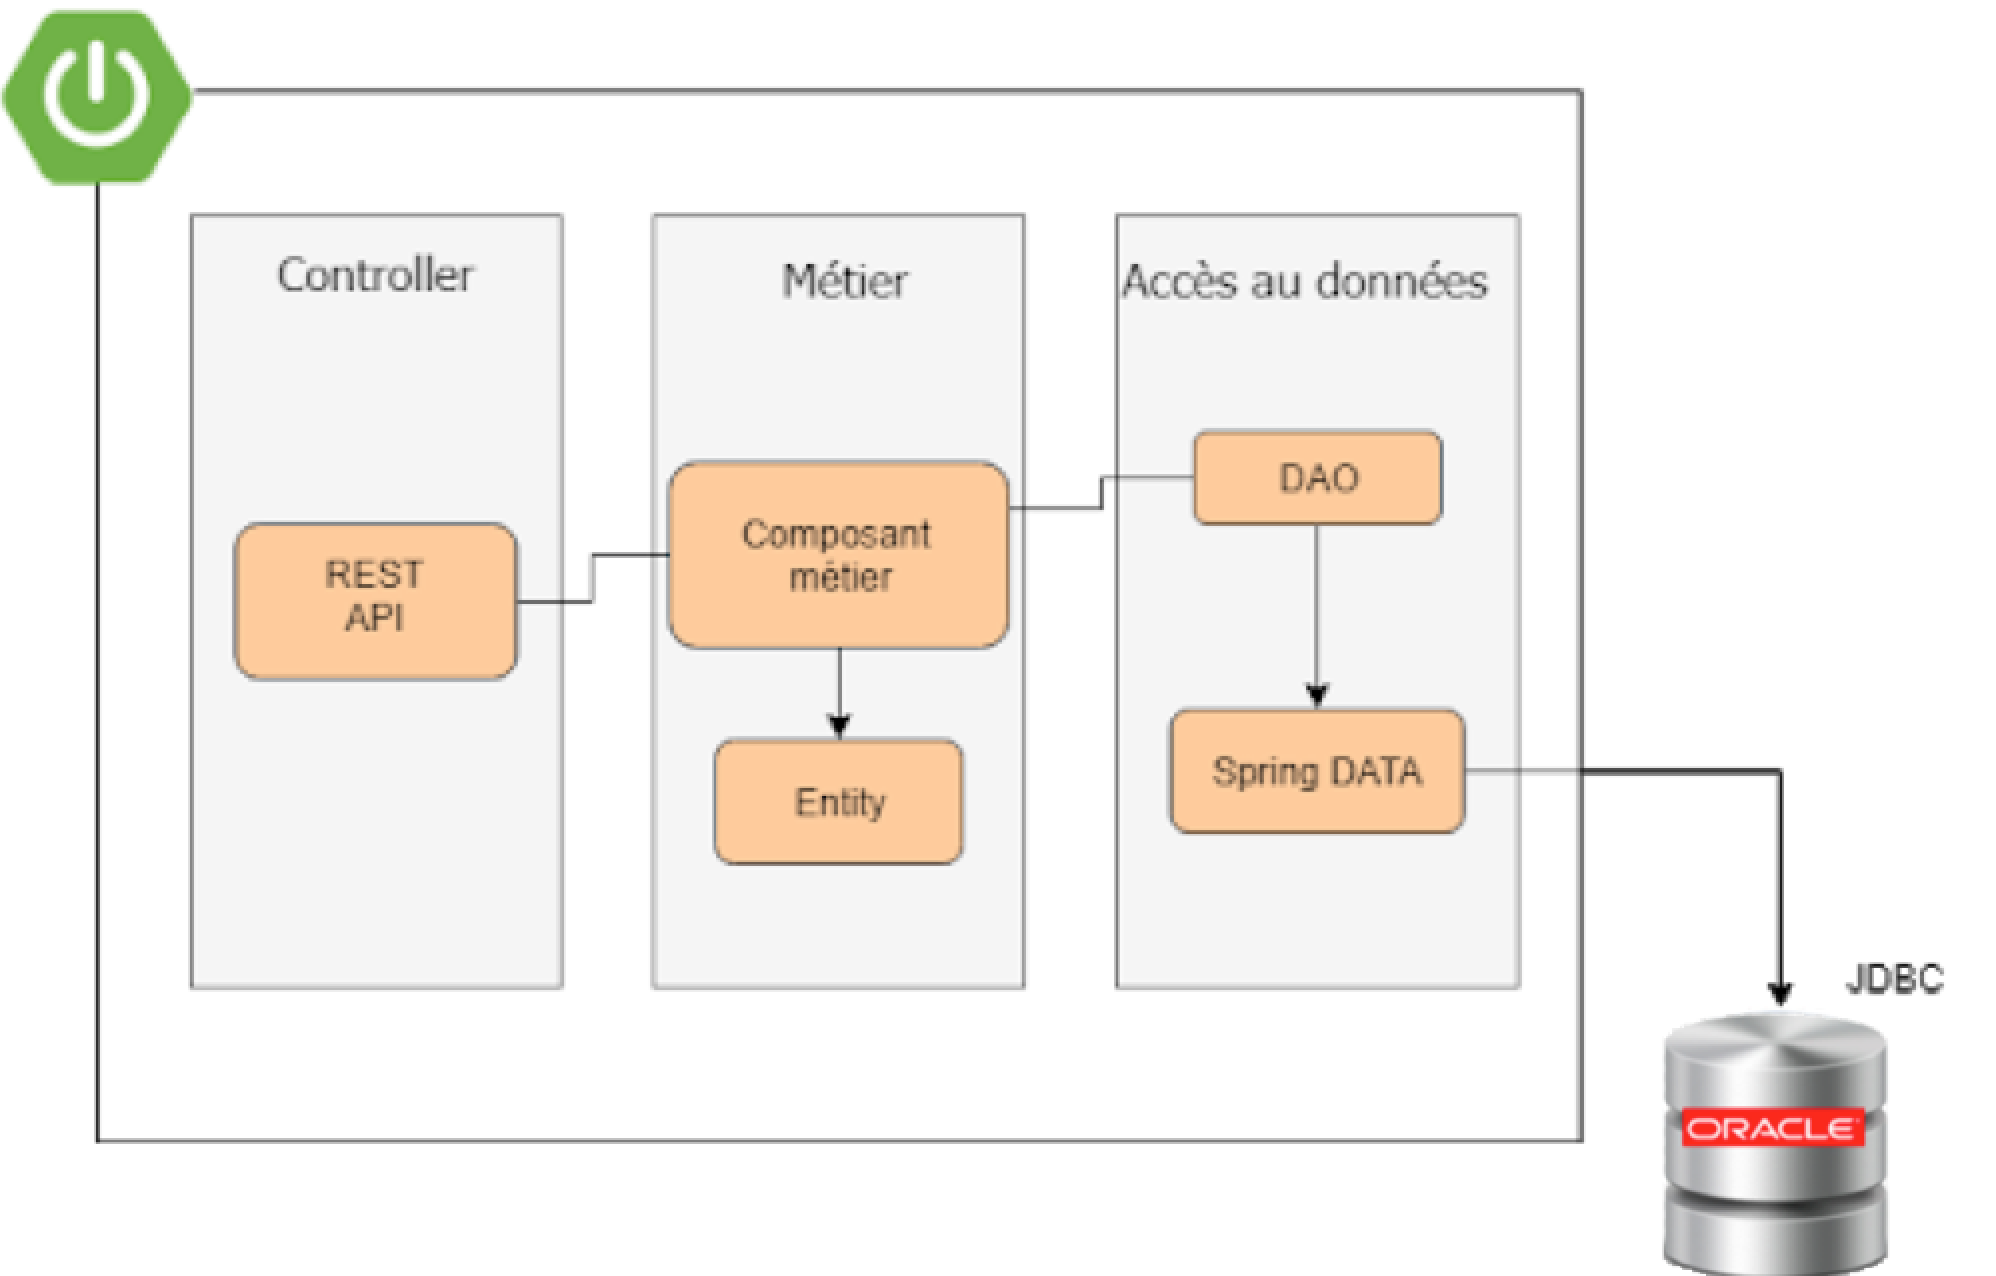
\includegraphics[width=1\textwidth]{chapitre3/Figures/spring.png}
  \caption{L'architecture serveur}
\end{figure}

L’architecture du Back-end se présente comme suit :
\begin{itemize}[label=\textbullet]
  \item La couche controller est la couche supérieure d'une application Web. Elle est responsable du traitement de l'entrée de l'utilisateur et renvoie la réponse correcte à l'utilisateur
  \item La couche métier correspond à la partie fonctionnelle de l’application, qui est responsable de l’implémentation de la « logique », décrivant les opérations que l’application opère sur les données en fonction des requêtes des utilisateurs, effectuées au travers de la couche controller.
  \item La couche accès aux données s’occupe de l’échange des informations entre le système qui gère la persistance des données et les objets de la couche métier.
\end{itemize}

\subsection{Communication Client/Serveur}
La mise en place d'une API permet d'opérer une séparation de responsabilités entre le client et le serveur. \\
Pour notre application, on a opté pour que l'interfaçage entre le client et le serveur se fait par REST, une API qui fait appel à des requêtes HTTP pour obtenir (GET), publier (POST), placer (PUT) et supprimer (DELETE) des données. [Voir Annexe B - REST API]

\begin{figure}[h!]  
 \centering
    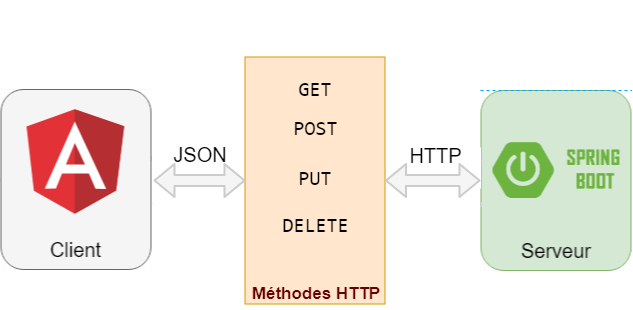
\includegraphics[width=1\textwidth]{chapitre3/Figures/rest.png}
  \caption{Communication Client/Serveur}
\end{figure}

